\section{Gradient micro-inertia and the high-wavenumber response}
\label{sec:microinertia}

Gradient micro-inertia accounts for spatial gradients of velocity in the kinetic energy. We examine the resulting high-wavenumber behaviour of the transverse branch and the associated strain-energy partition.

\subsection{Energy partition and the transverse-branch limit}
For Mindlin Form-II elasticity, the strain energy splits into classical and gradient parts, $W=W_c+W_g$, with $W_c=\tfrac12\int_\Omega\sigma_{ij}\varepsilon_{ij}\,\dif\Omega$ and $W_g=\tfrac12\int_\Omega\tau_{ijk}\eta_{ijk}\,\dif\Omega$. Along $\Gamma$--$X$, the gradient-energy fraction rises from $0.20\%$ at $\bar{k}=0.1$ to $16.49\%$ at $\bar{k}=1.0$ (Figure~\ref{fig:energy_microinertia}). The contribution of double-stress work increases as the wavelength becomes shorter.

\begin{figure*}[htbp]
\centering
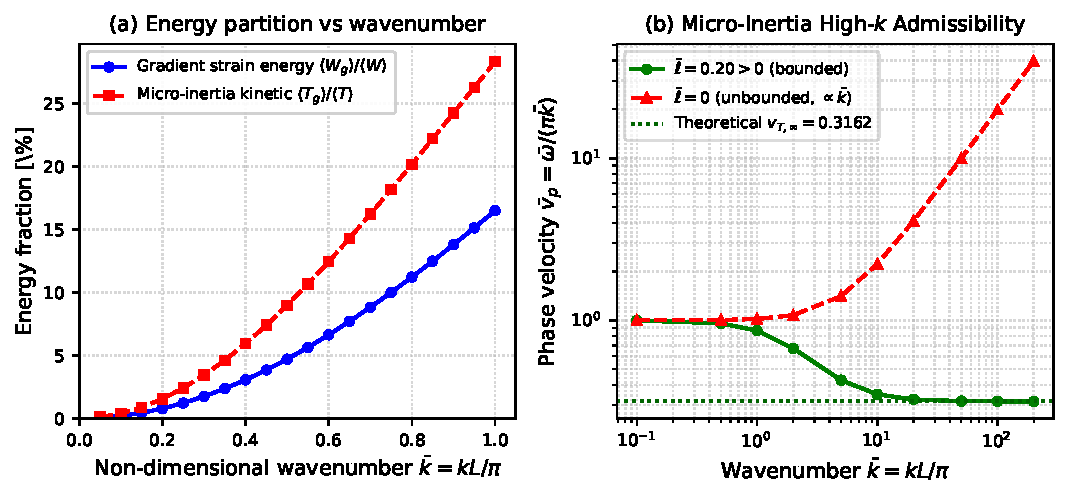
\includegraphics[width=\textwidth]{figures/fig13_energy_microinertia.pdf}
\caption{(a) Gradient-energy fraction $W_g/W$ versus wavenumber. (b) Transverse-branch phase velocity with and without gradient micro-inertia; the finite high-wavenumber limit is specific to the shear branch analyzed here}
\label{fig:energy_microinertia}
\end{figure*}

The transverse shear branch analyzed in Appendix~\ref{app:asymptotics} has the asymptotic limit
\begin{equation}
\begin{split}
\bar{v}_{T,\infty} &= \frac{\bar{l}_{\mathrm{eff}}}{\sqrt{10}\,\bar{\ell}_{\mathrm{i}}} \\
&= \frac{0.20}{\sqrt{10}\times0.20} = \frac{1}{\sqrt{10}} \approx 0.3162.
\end{split}
\label{eq:v_horizon_sec7}
\end{equation}
At $\bar{k}=200$, the computed phase speed with micro-inertia is $0.3163$, within $0.03\%$ of this asymptote. Without micro-inertia, the analytical branch relation grows without bound, and the computed phase speed reaches $39.75$ at $\bar{k}=200$. In Eq.~\eqref{eq:appA_vp}, the gradient stiffness and micro-inertia terms scale with $k^2$ in the numerator and denominator of $v_p^2$. Their ratio approaches a finite value. When $\ell_{\mathrm{i}}=0$, that denominator correction vanishes and the phase speed increases without bound. This result applies only to the transverse branch and constitutive model studied; it does not establish a speed bound for other branches or models.
